\section{Interfacce Utenti}
Di seguito sono descritte le interfacce utente con le quali l'utente deve interagire per usufruire del prodotto MyTalk.\\
\textit{Le interfacce descritte in questa sezione sono esclusivamente a scopo illustrativo.}

\subsection{GUI 1: Pagina accesso utente base}
La pagina accesso utente base è composta da due interfacce:
\begin{itemize}
\item \textbf{Login:} permette di effettuare l'autenticazione al sistema per accedere al sistema;
\item \textbf{Registrazione:} permette di accedere alla form di registrazione nel sistema.
\end{itemize}
Per impostazione di default\g~ la pagina iniziale al momento dell'accesso è aperta sull'interfaccia di login.

\subsubsection{GUI 1.1: Login}
Attraverso l'interfaccia di login l'utente può inserire le proprie credenziali (username e password) e accedere all'applicazione.
\begin{figure}[htbp]
\centering
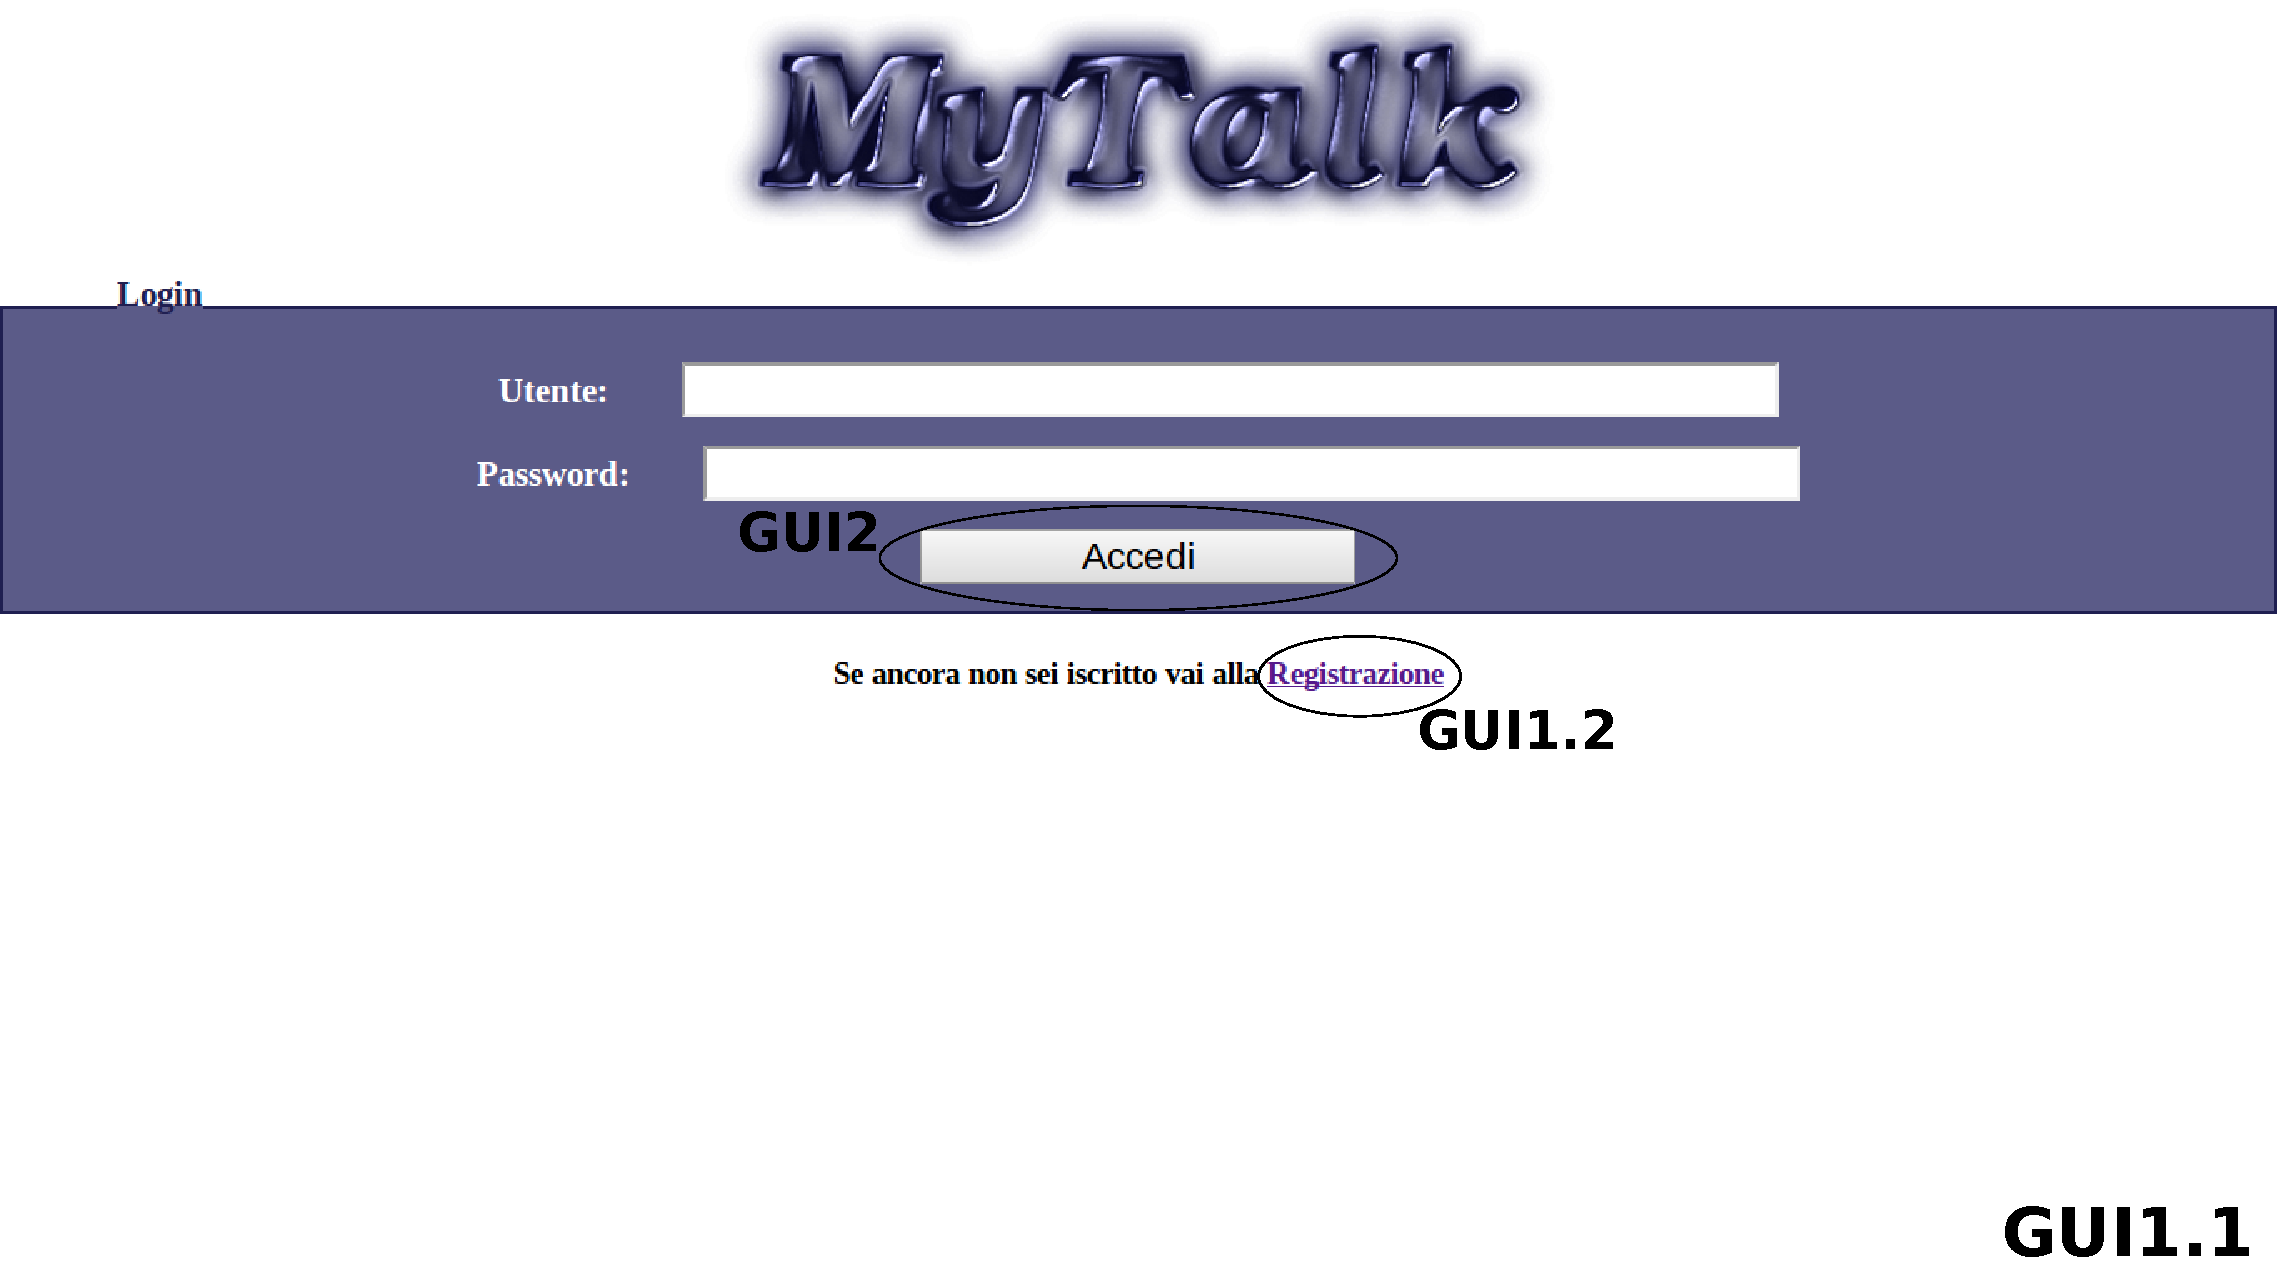
\includegraphics[scale=0.3]{\docsImg /interfacce/GUI1-1.pdf}
\caption{GUI 1.1 - Interfaccia di login.}
\end{figure}

\newpage
\subsubsection{GUI 1.2: Registrazione}
Attraverso l’interfaccia di registrazione l’utente può inserire le proprie credenziali per ottenere la possibilità di accedere all’applicazione. La struttura della form di registrazione è descritta nella figura \ref{figGUI12}.
\begin{figure}[htbp]
\centering
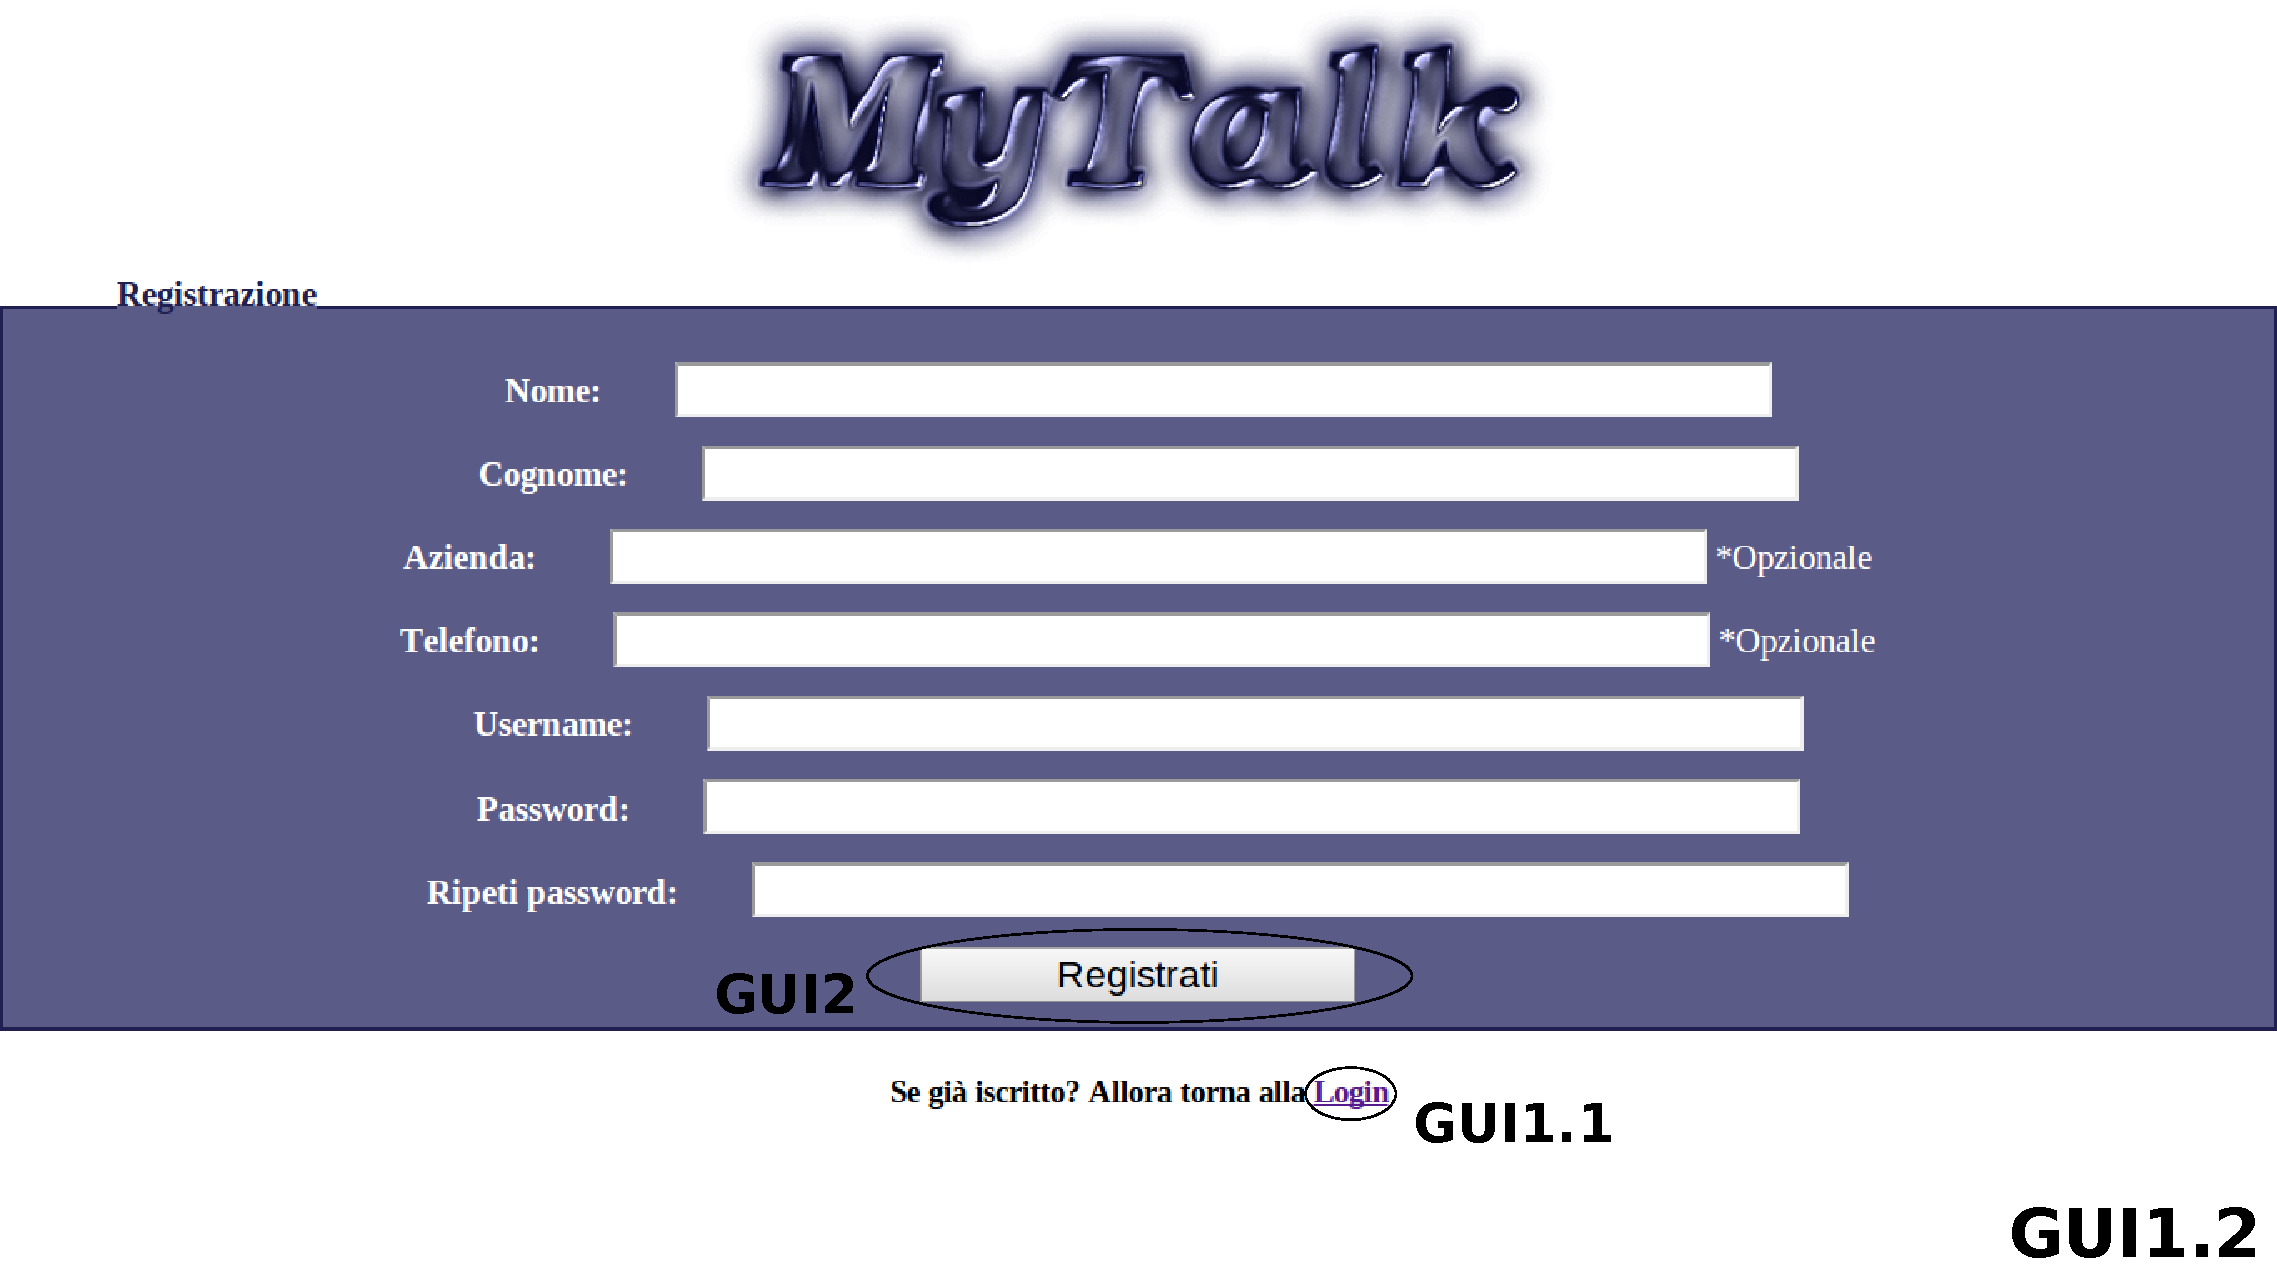
\includegraphics[scale=0.3]{\docsImg /interfacce/GUI1-2.pdf}
\label{figGUI12}
\caption{GUI 1.2 - Interfaccia di registrazione.}
\end{figure}

%\newpage
\subsection{GUI 2: Pagina principale utente base}
La pagina principale utente base presenta due parti fisse.\\
Nella prima vengono visualizzati i video in entrata e in uscita degli utenti in contatto durante una chiamata attiva. Se non ci sono comunicazioni attive, questa parte viene oscurata fino all'arrivo di una nuova trasmissione. Nella seconda, vengono visualizzati i dati principali dell'utente e viene offerta la possibilità di effettuare il logout e di scegliere tra una delle seguenti due interfacce:
\begin{itemize}
\item \textbf{Comunicazioni:} permette di gestire le comunicazioni;
\item \textbf{Dati Utente:} permette di visualizzare e modificare le credenziali dell’utente.
\end{itemize} 
\begin{figure}[h!tbp]
\centering
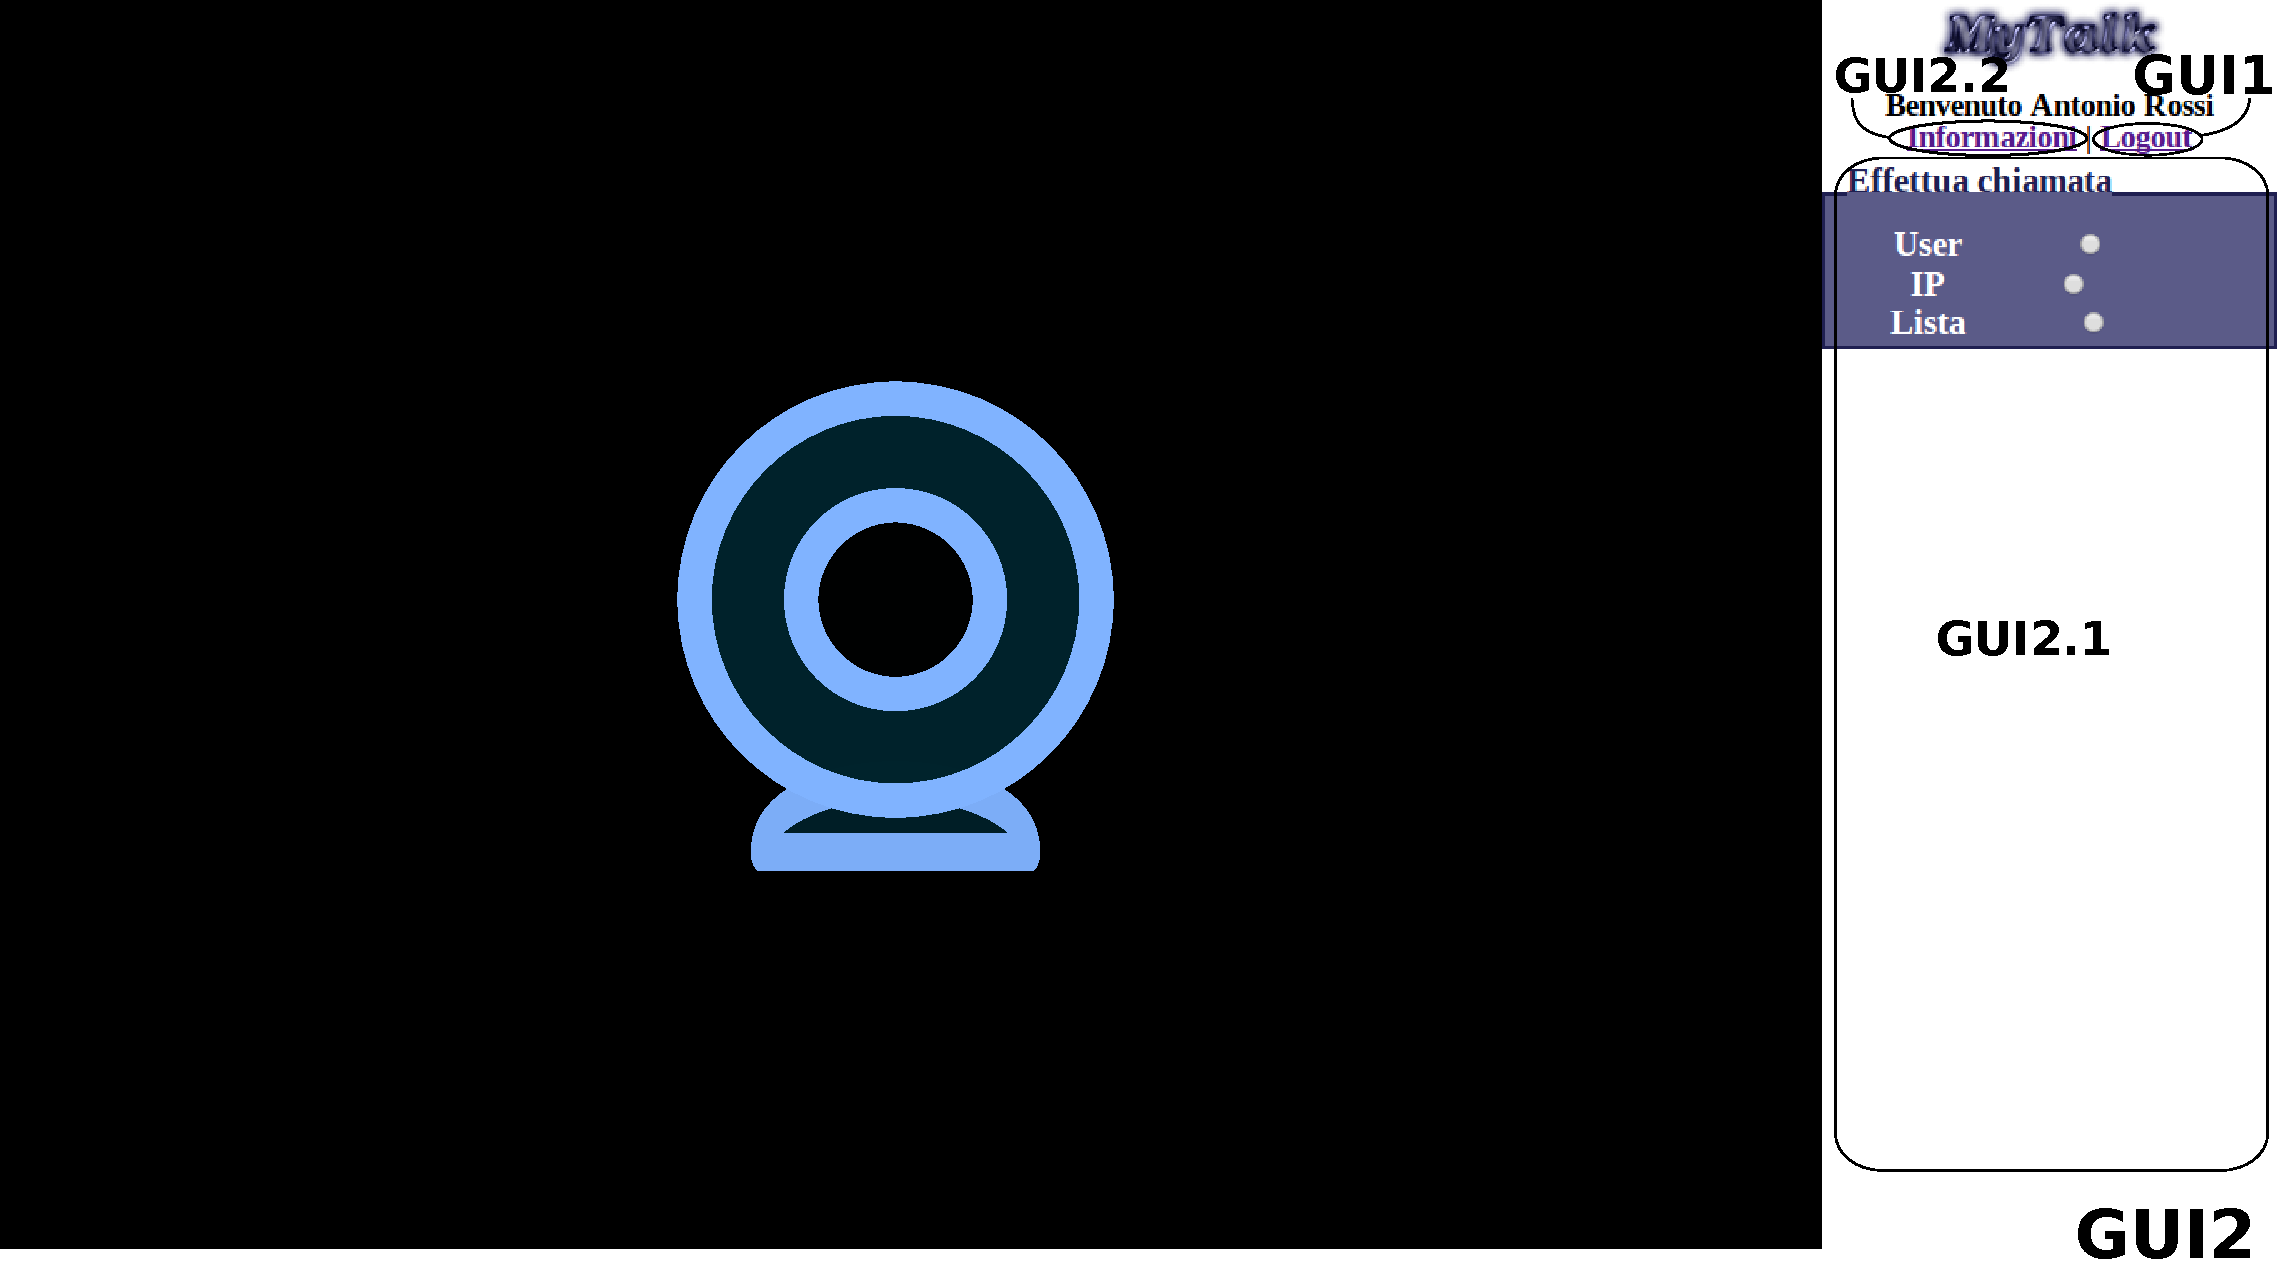
\includegraphics[scale=0.3]{\docsImg /interfacce/GUI2.pdf}
\caption{GUI 2 - Pagina principale utente.}
\end{figure}

\subsubsection{GUI 2.1: Comunicazione}
La seguente interfaccia è composta da vari pannelli che permettono di interagire con le comunicazioni in entrata ed uscita.
\begin{itemize}
\item \textbf{Effettua chiamata:} permette di decidere il metodo di selezione dell’utente da chiamare e successivamente di chiamare l’utente scelto.
\item \textbf{Chiamata in arrivo:} questo pannello appare al momento dell’arrivo di una richiesta di comunicazione e permette di decidere se accettarla o rifiutarla.
\item \textbf{Informazioni chiamata:} si presenta quando è presente una chiamata attiva e visualizza i dati della comunicazione e permette di terminare la conversazione.
\item \textbf{Chiamata terminata:} si presenta al termine di tutte le comunicazione con lo scopo di valutare la qualità del servizio.
\end{itemize} 

\subsubsection{GUI 2.1.1: Effettua chiamata}
Il pannello si espande permettendo di scegliere:
\begin{itemize}
\item \textbf{Chiamata per IP\g}
\item \textbf{Chiamata per username}
\item \textbf{Chiamata per scelta utente da lista}
\end{itemize} 
Una volta effettuata la scelta si espande e viene visualizzata la form richiesta dalla quale è possibile inviare una richiesta di comunicazione.\\
Il pannello non è accessibile durante una comunicazione in corso fino a dopo aver effettuato la valutazione.
\begin{figure}[htbp]
\centering
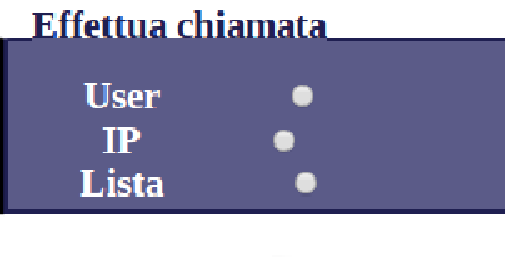
\includegraphics[scale=0.5]{\docsImg /interfacce/GUI2-1-1.pdf}
\caption{GUI 2.1.1 - Pannello effettua chiamata.}
\end{figure}

\subsubsection{GUI 2.1.1.1 Chiamata per IP}
Il pannello si espande e presenta una form per l’inserimento dell’indirizzo IP\g.
\begin{figure}[htbp]
\centering
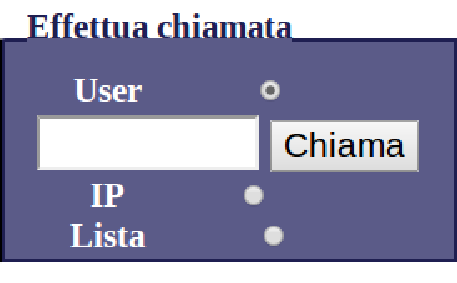
\includegraphics[scale=0.5]{\docsImg /interfacce/GUI2-1-1-1.pdf}
\caption{GUI 2.1.1.1 - Pannello effettua chiamata attraverso IP\g.}
\end{figure}

\subsubsection{GUI 2.1.1.2 Chiamata per Username}
Il pannello si espande e presenta una form per l’inserimento dello username.
\begin{figure}[htbp]
\centering
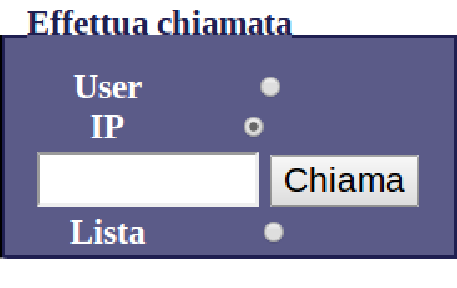
\includegraphics[scale=0.5]{\docsImg /interfacce/GUI2-1-1-2.pdf}
\caption{GUI 2.1.1.2 - Pannello effettua chiamata attraverso username.}
\end{figure}

\subsubsection{GUI 2.1.1.3 Chiamata per scelta utente da lista}
Il pannello si espande e permette di scegliere dalla lista di tutti gli utenti online l’utente da chiamare.
\begin{figure}[htbp]
\centering
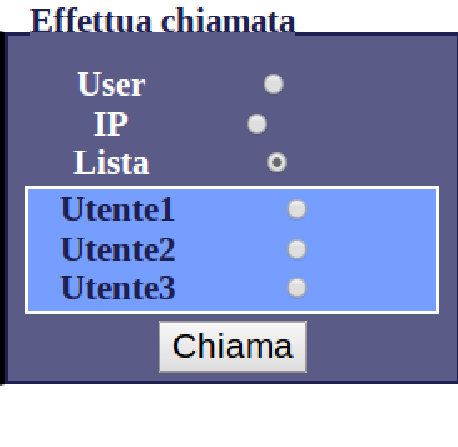
\includegraphics[scale=0.5]{\docsImg /interfacce/GUI2-1-1-3.pdf}
\caption{GUI 2.1.1.3 - Pannello effettua chiamata attraverso scelta da lista.}
\end{figure}

%\newpage
\subsubsection{GUI 2.1.2 Chiamata in entrata}
Il pannello appare all’arrivo di una richiesta di comunicazione in entrata e permette all’utente di scegliere se accettare o rifiutare di rispondere.
\begin{figure}[htbp]
\centering
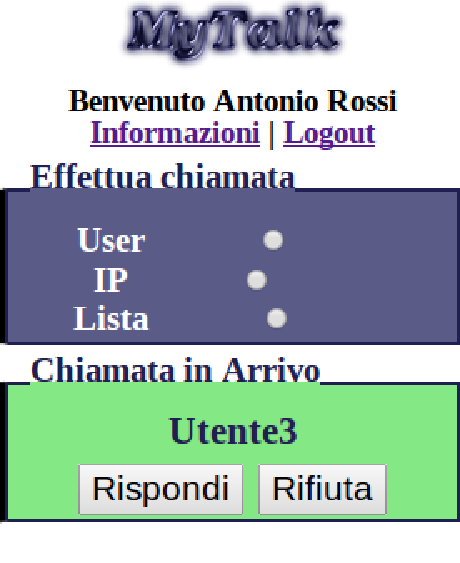
\includegraphics[scale=0.5]{\docsImg /interfacce/GUI2-1-2.pdf}
\caption{GUI 2.1.2 - Pannello di chiamata in entrata.}
\end{figure}

\subsubsection{GUI 2.1.3 Informazioni chiamata}
Il pannello informazioni chiamata visualizza durata, latenza, byte inviati e la velocità della comunicazione. Infine permette di terminare la conversazione.
\begin{figure}[htbp]
\centering
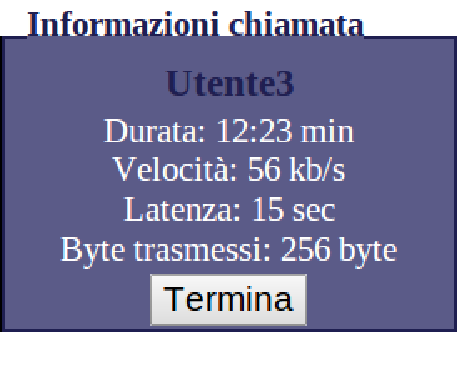
\includegraphics[scale=0.5]{\docsImg /interfacce/GUI2-1-3.pdf}
\caption{GUI 2.1.3 - Pannello informazioni chiamata.}
\end{figure}

\subsubsection{GUI 2.1.4 Chiamata terminata}
Il pannello si attiva al termine della comunicazione allo scopo di valutare la qualità della conversazione. La valutazione di qualità avviene su una scala da 1 a 5.
\begin{figure}[htbp]
\centering
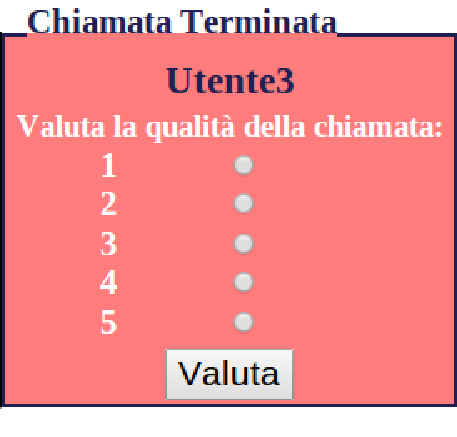
\includegraphics[scale=0.5]{\docsImg /interfacce/GUI2-1-4.pdf}
\caption{GUI 2.1.4 - Pannello chiamata terminata.}
\end{figure}

\subsubsection{GUI 2.2: Dati utente}
La seguente interfaccia visualizza le informazioni dell’utente e permette di modificarne i dati attraverso due pannelli:
\begin{itemize}
\item \textbf{Visualizza dati}
\item \textbf{Modifica dati}
\end{itemize}
All’apertura di questa interfaccia si apre di default\g~ il pannello visualizza dati.
\begin{figure}[htbp]
\centering
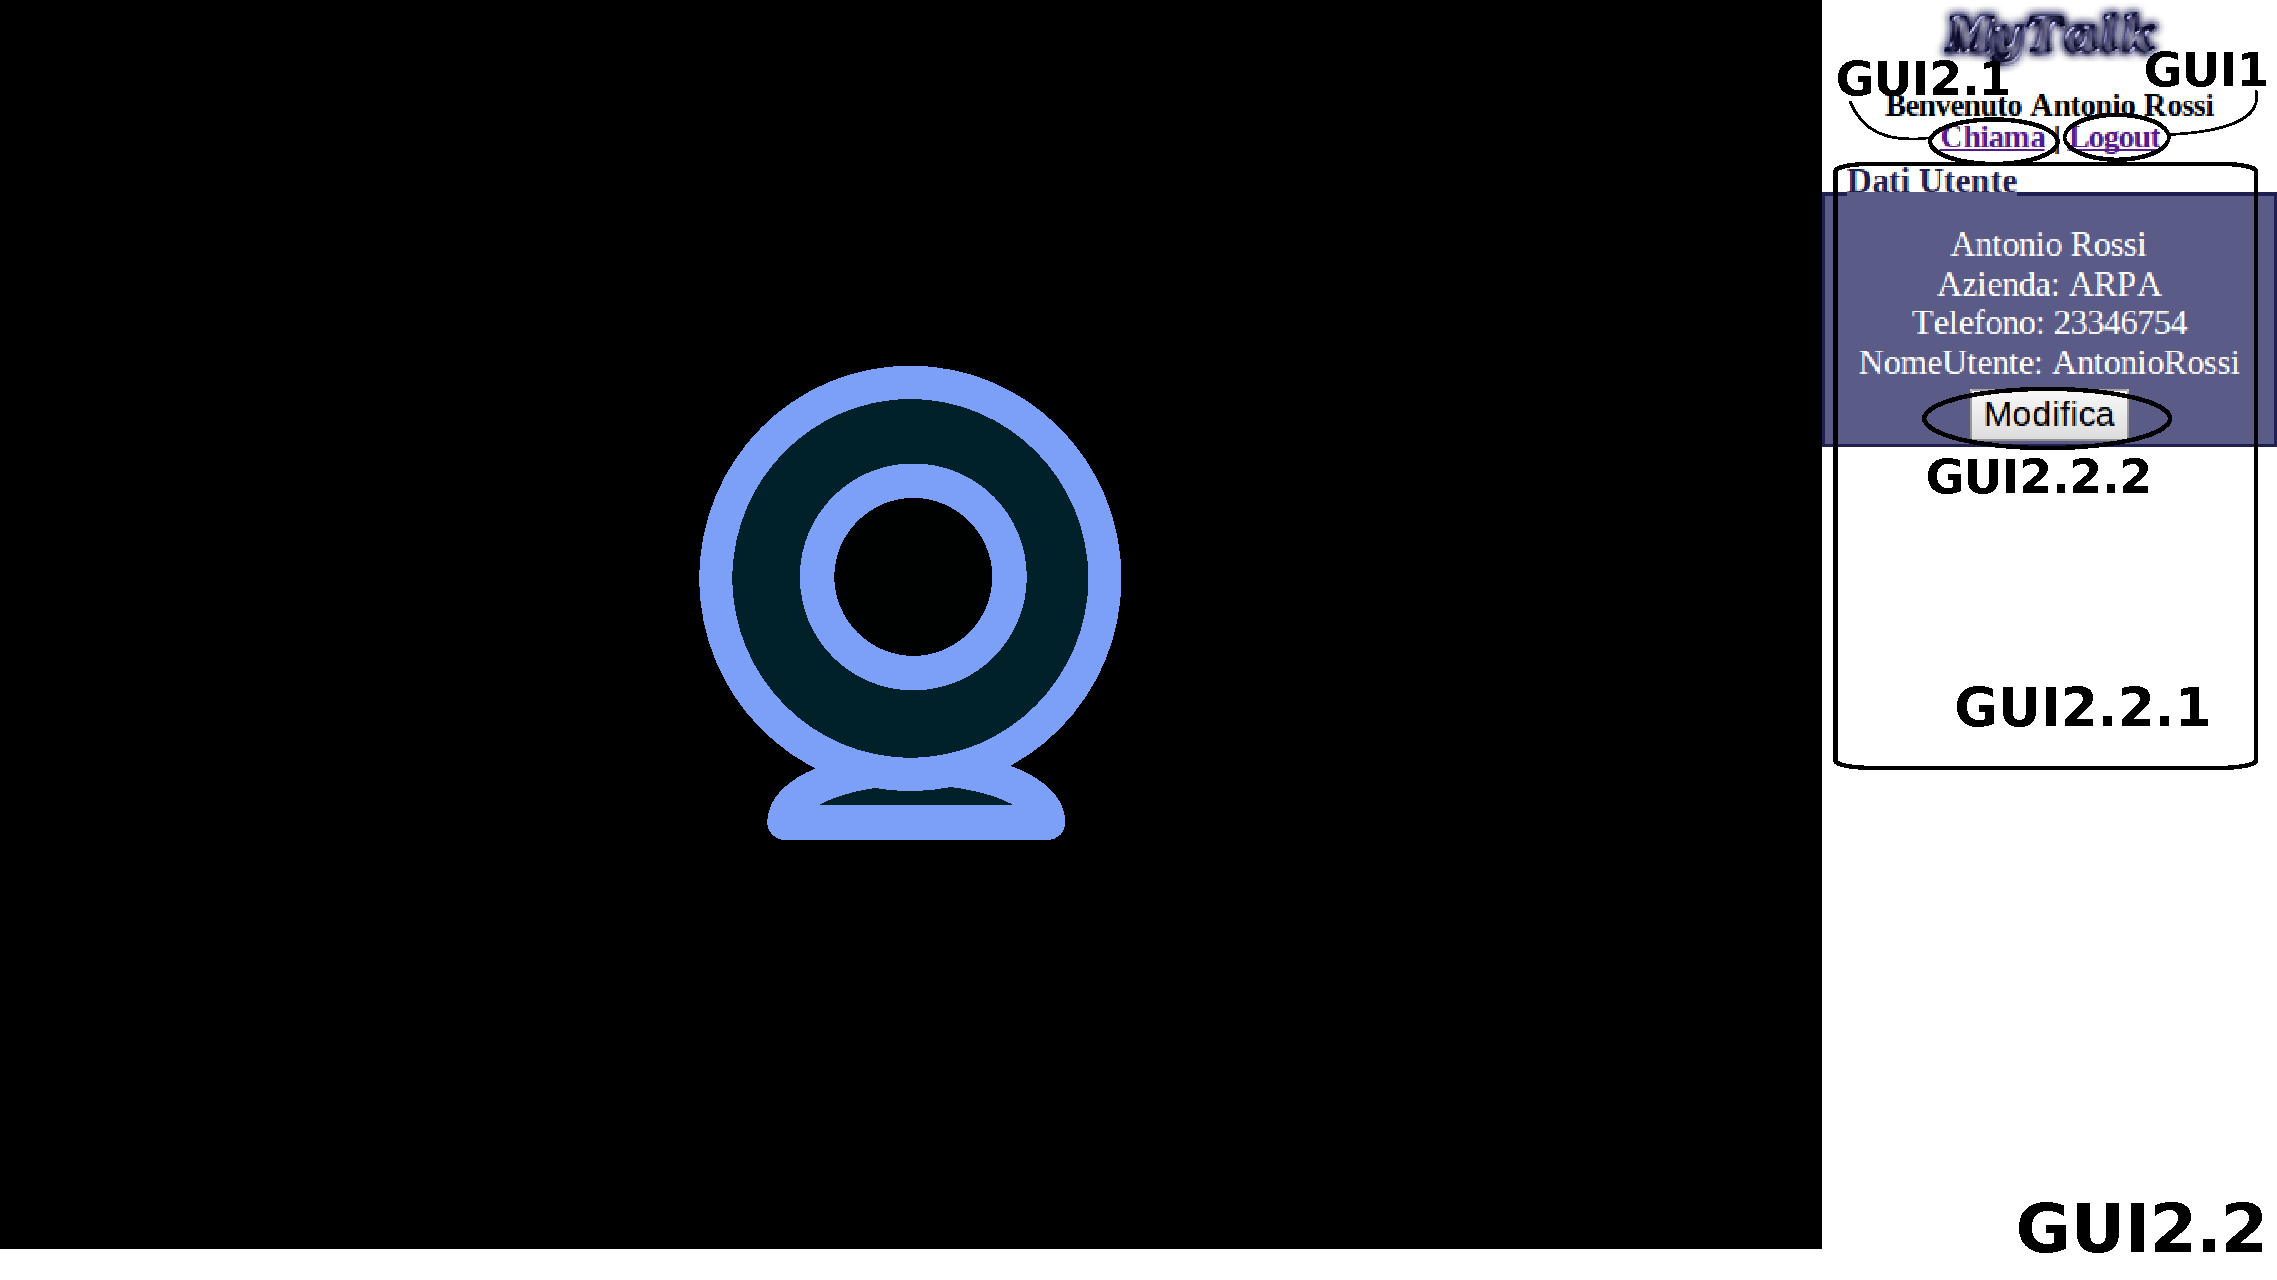
\includegraphics[scale=0.3]{\docsImg /interfacce/GUI2-2.pdf}
\caption{GUI 2.2 - Dati utente.}
\end{figure}

\subsubsection{GUI 2.2.1: Visualizza dati}
Il pannello che visualizza i dati mostra le informazioni dell’utente e chiede all’utente se desidera modificarle.

\newpage
\subsubsection{GUI 2.2.2: Modifica dati}
Il pannello che visualizza e modifica i dati dell'utente.
\begin{figure}[htbp]
\centering
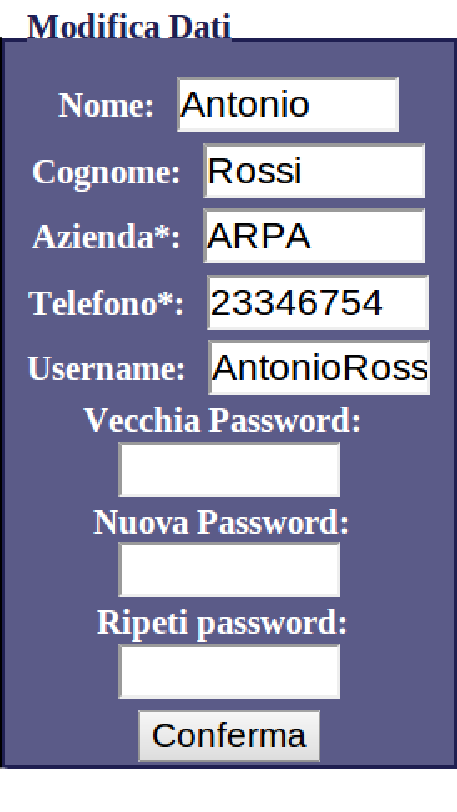
\includegraphics[scale=0.5]{\docsImg /interfacce/GUI2-2-2.pdf}
\caption{GUI 2.2.2 - Pannello modifica dati.}
\end{figure}

%\newpage
\subsection{GUI 3: Pagina accesso amministratore}
La pagina di accesso amministratore a differenza dell’interfaccia di accesso utente base presenta una sola interfaccia di login, solo un utente predefinito può accedere alla pagina principale amministratore.
\begin{figure}[htbp]
\centering
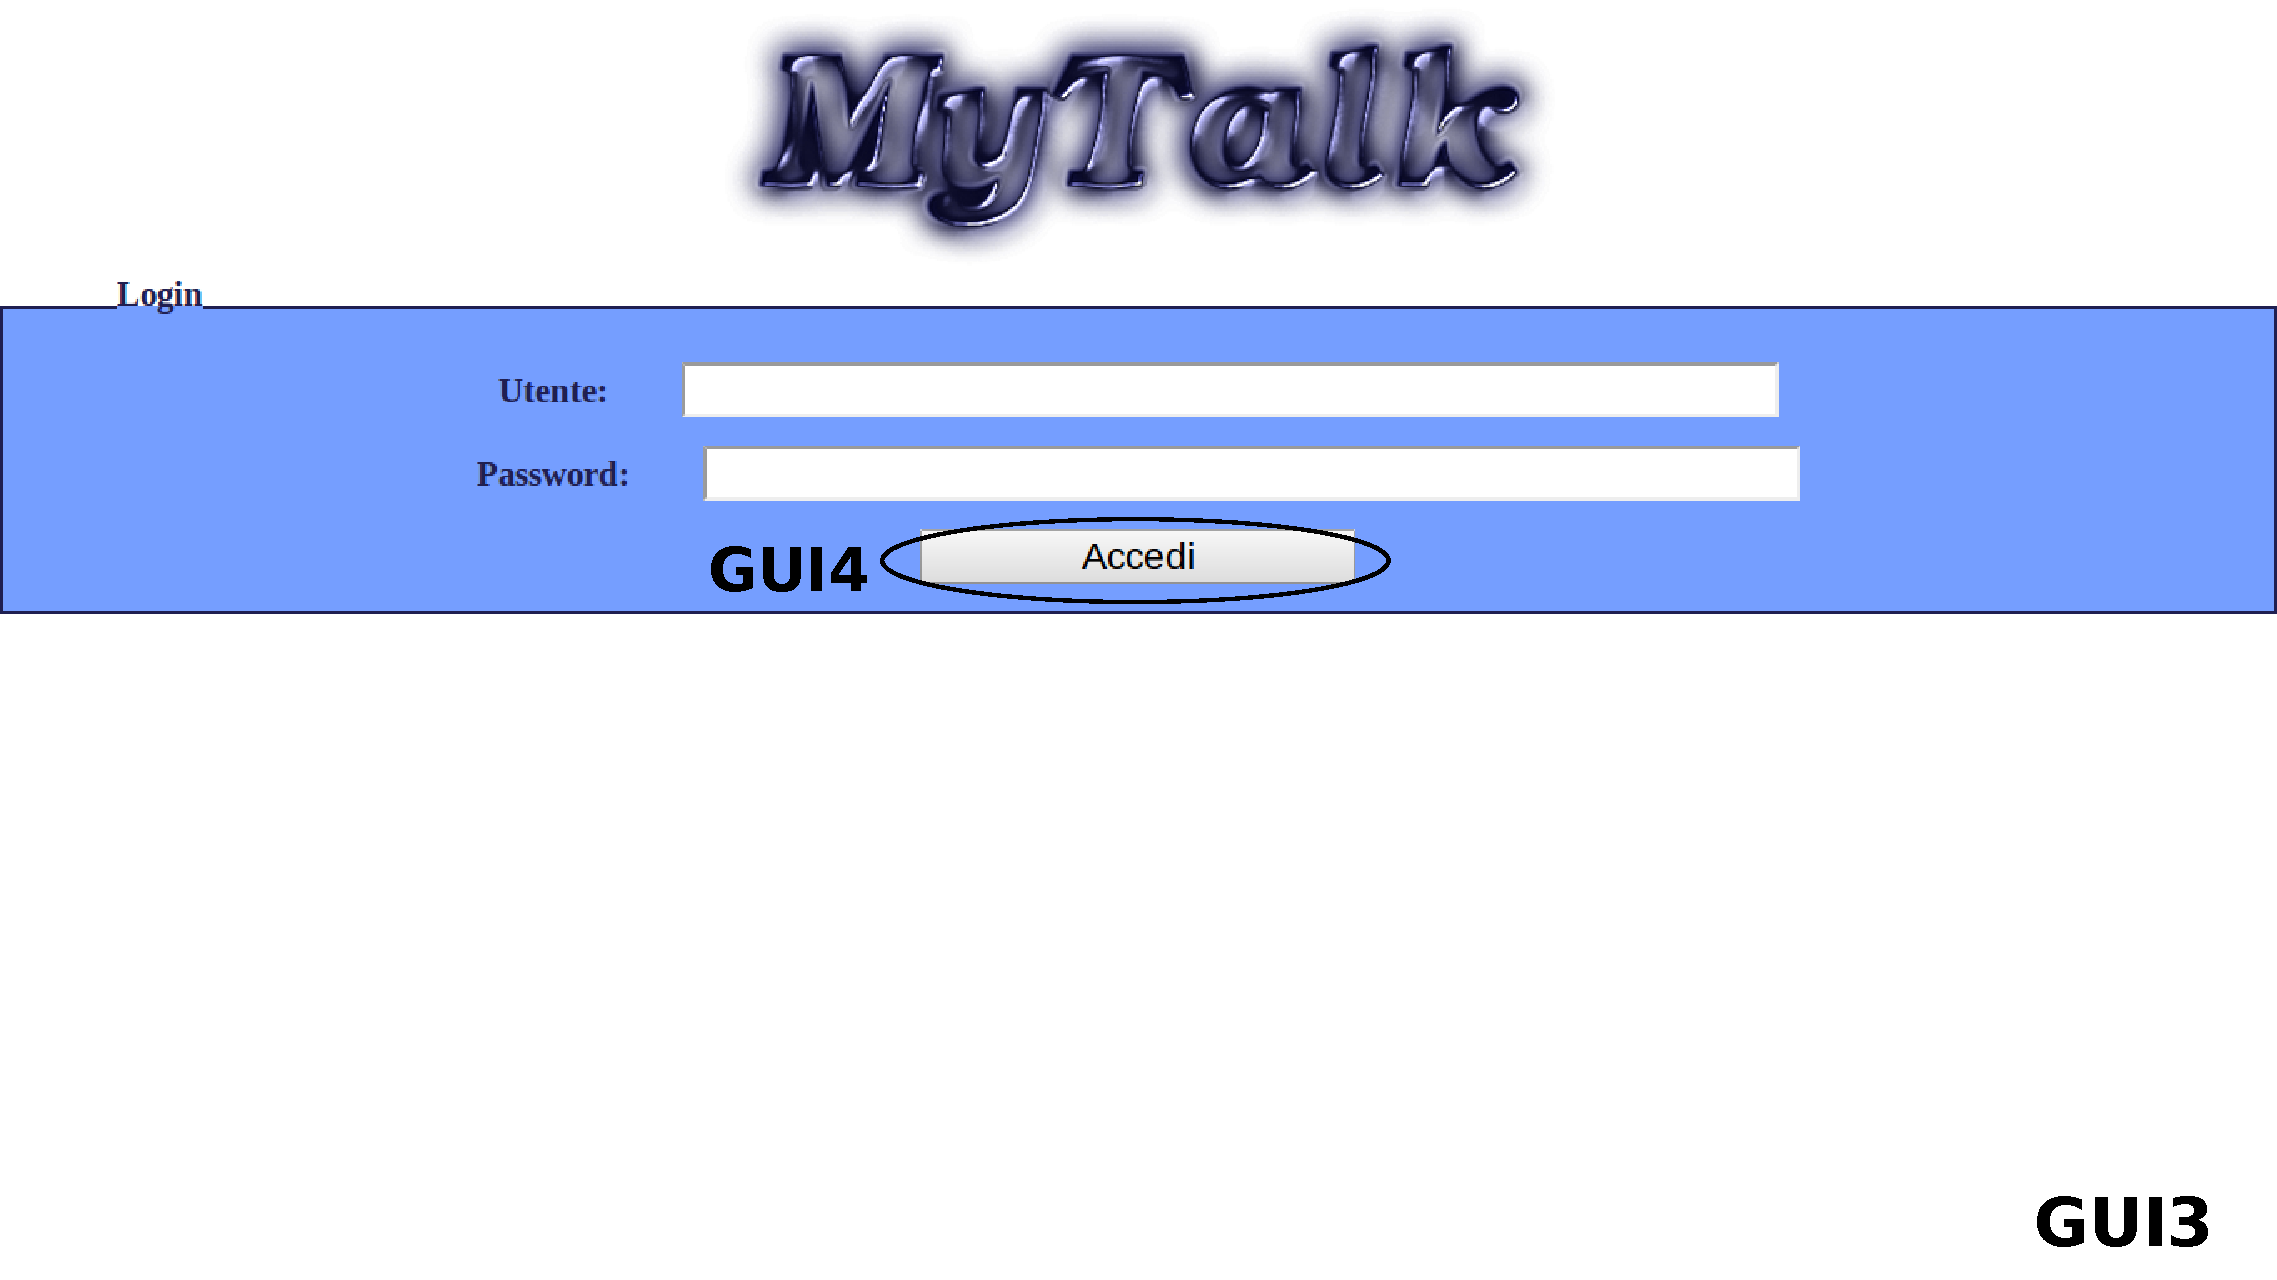
\includegraphics[scale=0.3]{\docsImg /interfacce/GUI3.pdf}
\caption{GUI 3 - Pagina accesso amministratore.}
\end{figure}

\newpage
\subsection{GUI 4: Pagina principale amministratore}
La pagina principale amministratore è divisa in due parti. Una è la lista delle chiamate con relative informazioni  che l’amministratore vuole visualizzare, l’altra è la parte dalla quale l’amministratore può, tramite un pannello, filtrare le chiamate o effettuare il logout.\\
La lista contiene tutte le informazioni relative alle telefonate: mittente, destinatario, latenza, byte trasmessi, giudizio, velocità, durata e data.
\begin{figure}[htbp]
\centering
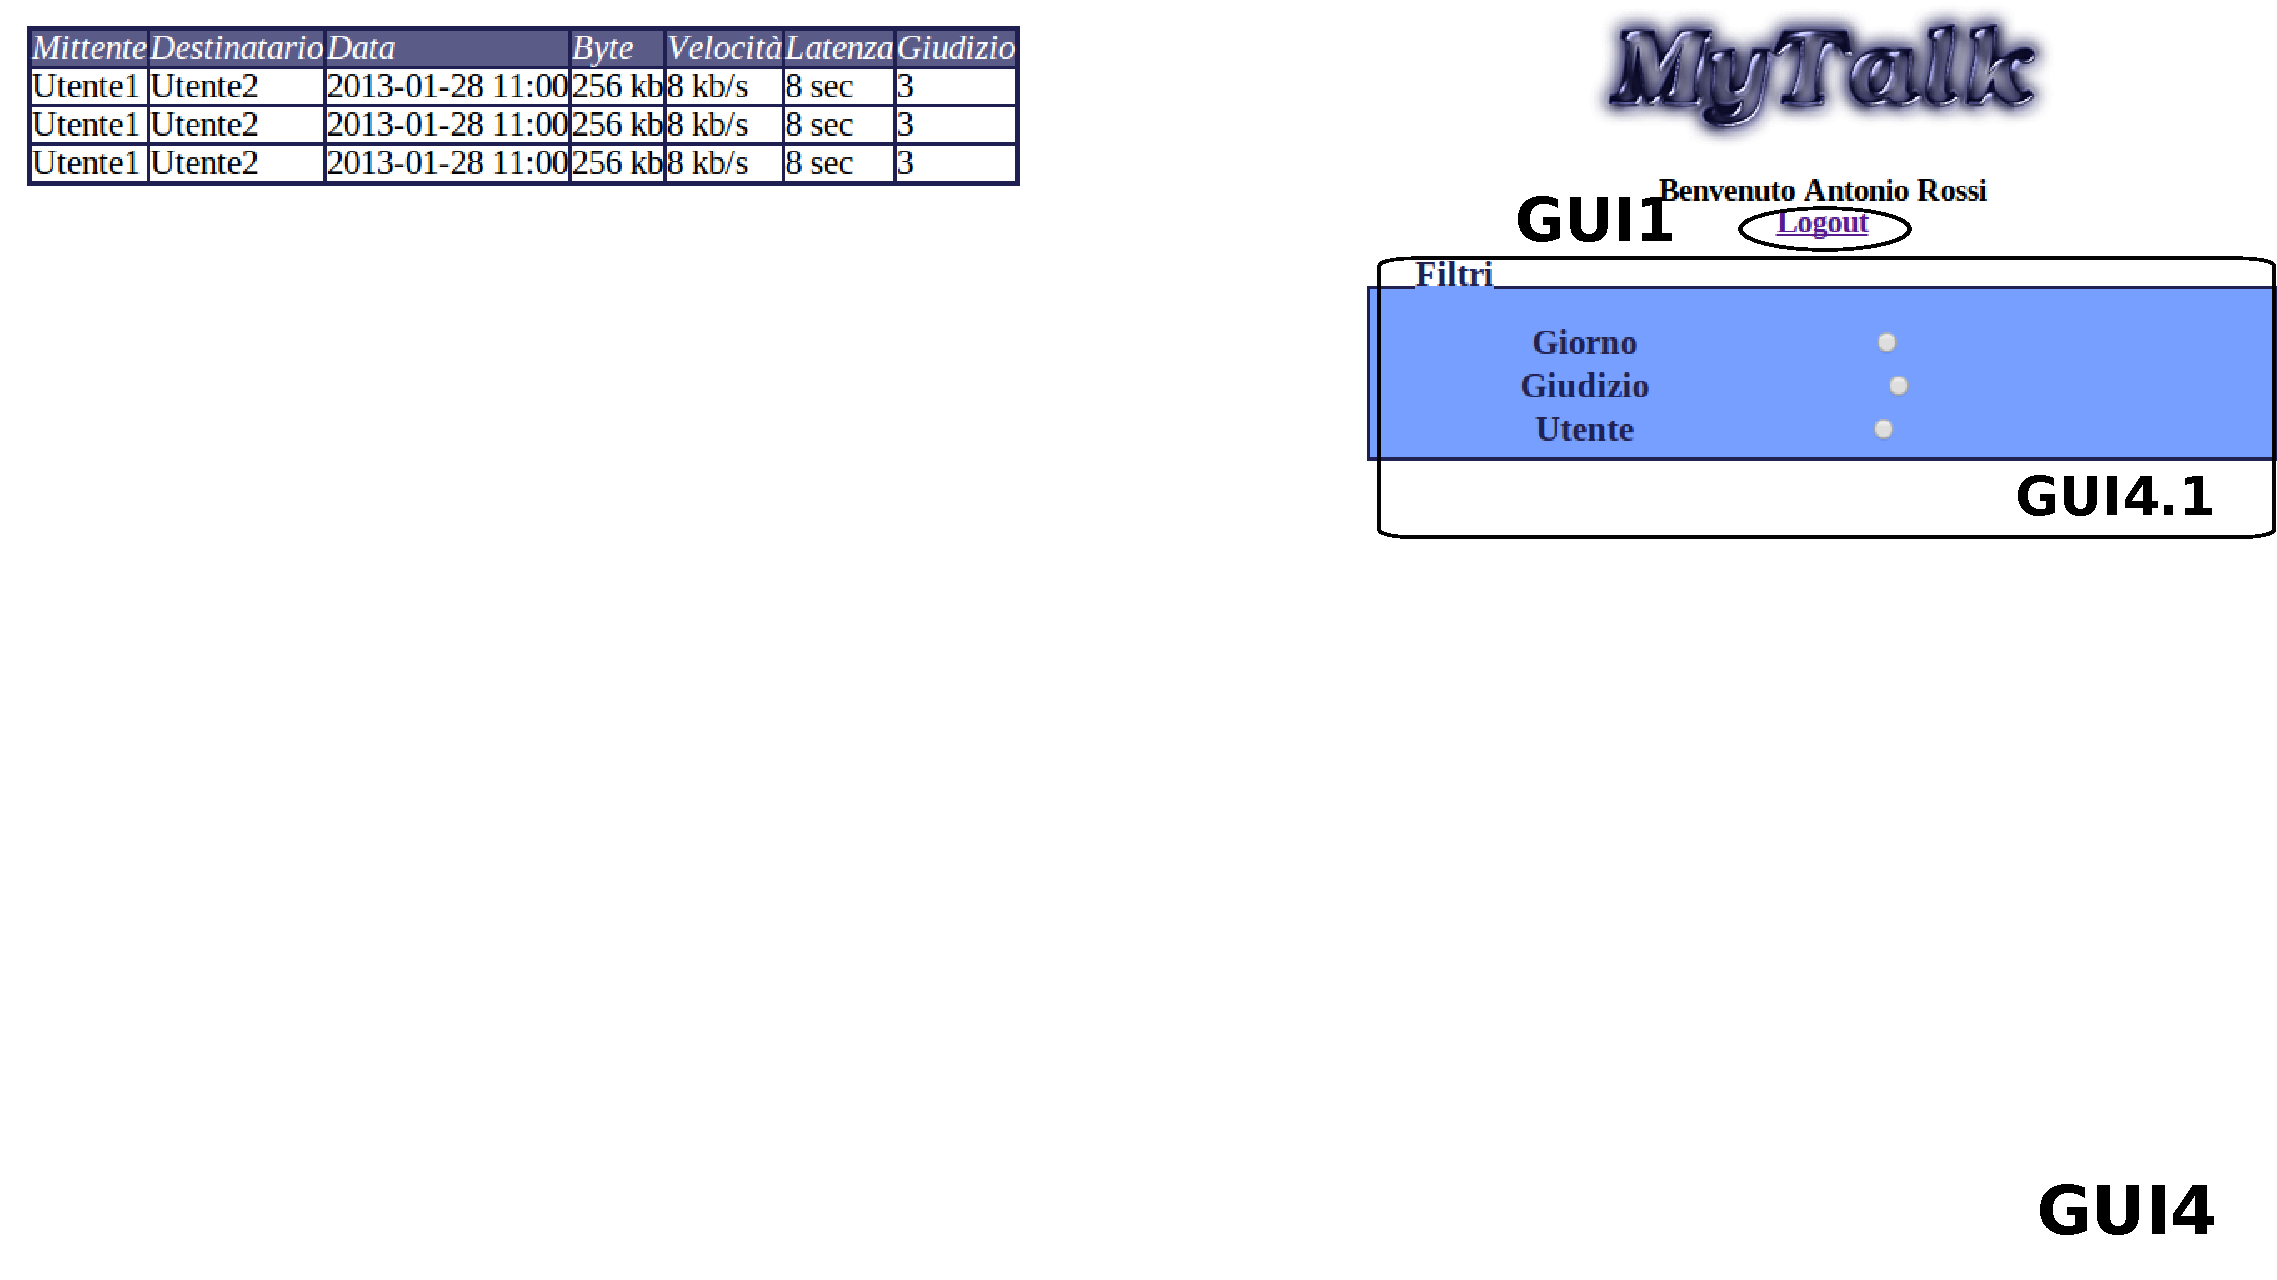
\includegraphics[scale=0.3]{\docsImg /interfacce/GUI4.pdf}
\caption{GUI 4 - Pagina principale amministratore.}
\end{figure}

\subsubsection{GUI 4.1 Filtro}
Il pannello filtro permette all’amministratore di selezionare in che modo effettuare la scelta del filtro. Ci possono essere tre possibili filtri:
\begin{itemize}
\item Per giorno
\item Per giudizio
\item Per utente
\end{itemize}

\subsubsection{GUI 4.1.1 Filtro per giorno}
Il pannello si espande e permette di selezionare il giorno da filtrare.
\begin{figure}[htbp]
\centering
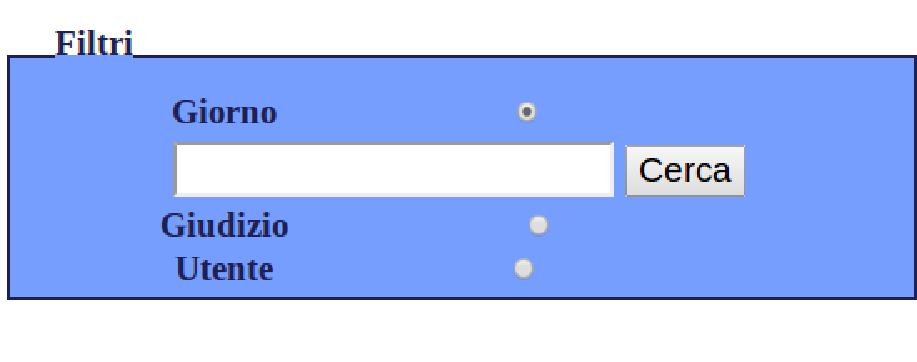
\includegraphics[scale=0.5]{\docsImg /interfacce/GUI4-1-1.pdf}
\caption{GUI 4.1.1 - Pannello filtro per giorno.}
\end{figure}

\subsubsection{GUI 4.1.2 Filtro per giudizio}
Il pannello si espande e permette di selezionare il giudizio da filtrare. 
\begin{figure}[htbp]
\centering
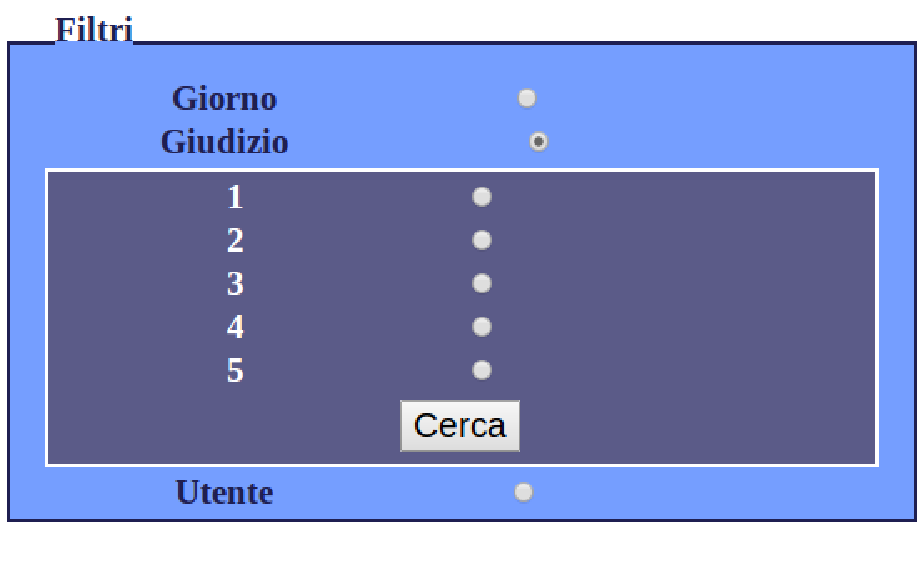
\includegraphics[scale=0.5]{\docsImg /interfacce/GUI4-1-2.pdf}
\caption{GUI 4.1.2 - Pannello filtro per giudizio.}
\end{figure}

\subsubsection{GUI 4.1.3 Filtro per utente}
Il pannello si espande e permette di selezionare in che modo selezionare l’utente da filtrare. Le possibilità sono tre: 
\begin{itemize}
\item Scelta per IP\g
\item Scelta per username
\item Scelta da lista
\end{itemize}
\begin{figure}[htbp]
\centering
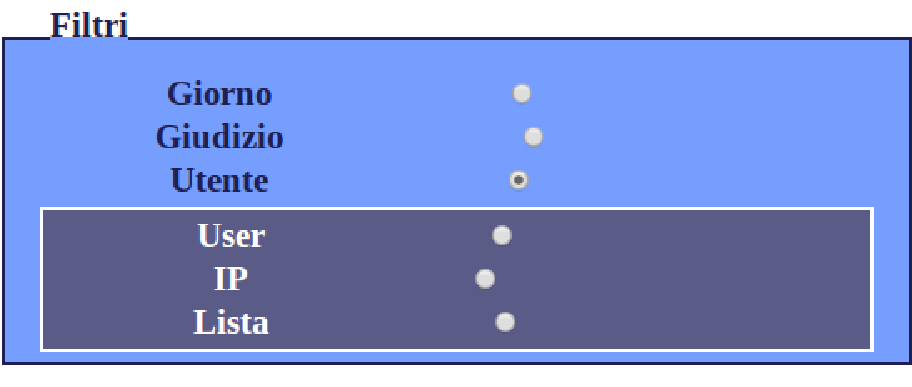
\includegraphics[scale=0.5]{\docsImg /interfacce/GUI4-1-3.pdf}
\caption{GUI 4.1.3 - Pannello filtro per utente.}
\end{figure}

\subsubsection{GUI 4.1.3.1 Filtro per utente da IP}
Il pannello si espande e presenta una form per l’inserimento dell’indirizzo IP\g.
\begin{figure}[htbp]
\centering
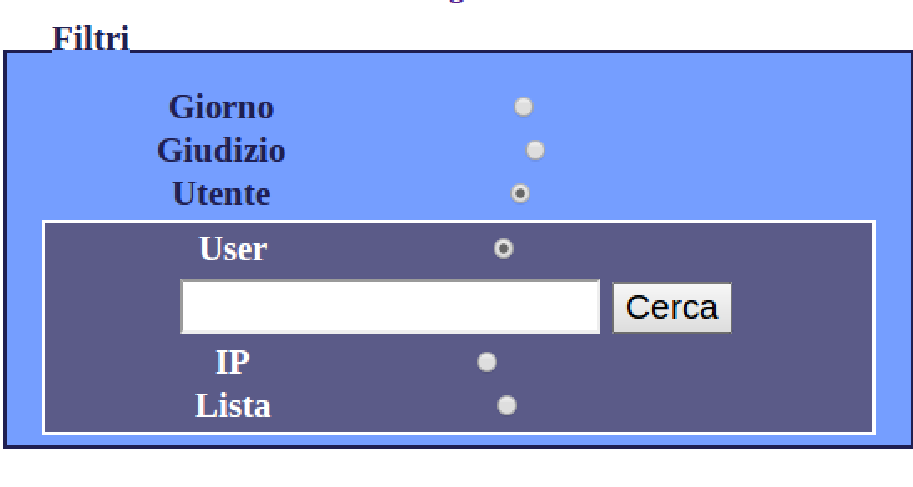
\includegraphics[scale=0.5]{\docsImg /interfacce/GUI4-1-3-1.pdf}
\caption{GUI 4.1.3.1 - Pannello filtro per utente da IP.}
\end{figure}

\subsubsection{GUI 4.1.3.2 Filtro per utente da username}
Il pannello si espande e presenta una form per l’inserimento dello username.
\begin{figure}[htbp]
\centering
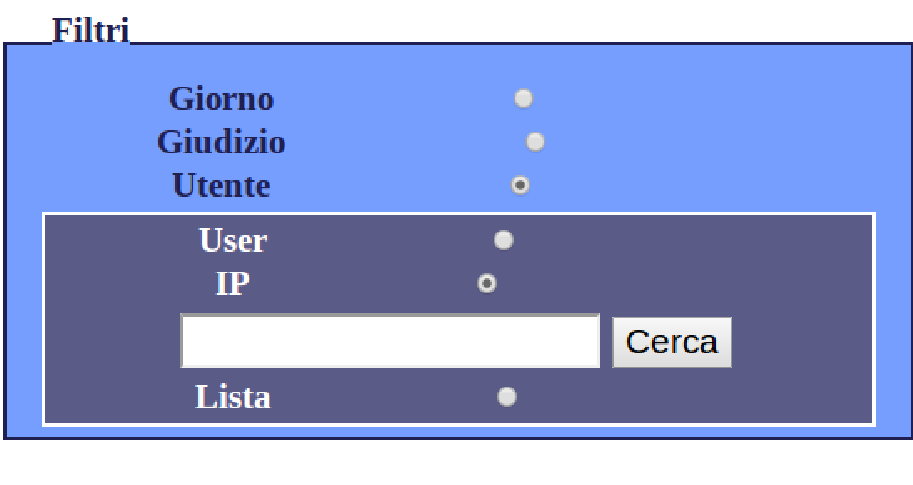
\includegraphics[scale=0.5]{\docsImg /interfacce/GUI4-1-3-2.pdf}
\caption{GUI 4.1.3.2 - Pannello filtro per utente da username.}
\end{figure}

\newpage
\subsubsection{GUI 4.1.3.3 Filtro per utente da lista}
Il pannello si espande permette di scegliere dalla lista di tutti gli utenti online l’utente da chiamare.
\begin{figure}[htbp]
\centering
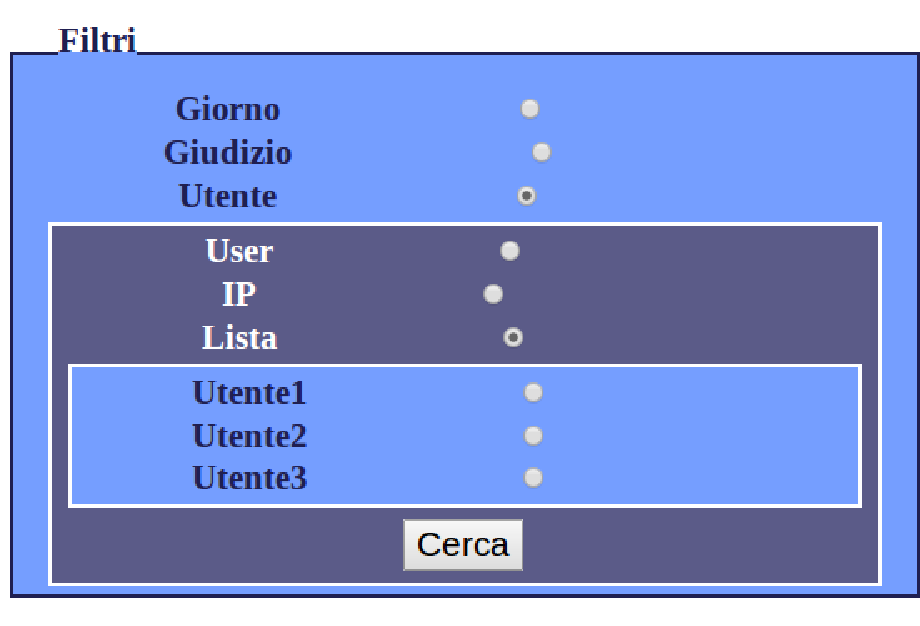
\includegraphics[scale=0.5]{\docsImg /interfacce/GUI4-1-3-3.pdf}
\caption{GUI 4.1.3.3 - Pannello filtro per utente da lista.}
\end{figure}